\documentclass[aspectratio=168, 10pt] {beamer}
\usepackage[utf8]{inputenc}
\usepackage[
  main=english, %% By using `czech` or `slovak` as the main locale
                %% instead of `english`, you can typeset the
                %% presentation in either Czech or Slovak,
                %% respectively.
  czech, slovak %% The additional keys allow foreign texts to be
]{babel}        %% typeset as follows:
%%
%%   \begin{otherlanguage}{czech}   ... \end{otherlanguage}
%%   \begin{otherlanguage}{slovak}  ... \end{otherlanguage}
%%
%% These macros specify information about the presentation
\title{Daylighting With Skylights in Different Climates:} %% that will be typeset on the
\subtitle{Creating Cost Saving Comfortable Infrastructure.} %% title page.
\author{Samara Elling}
%% These additional packages are used within the document:
\usepackage{ragged2e}  % `\justifying` text
\usepackage{booktabs}  % Tables
\usepackage{tabularx}
\usepackage{tikz}      % Diagrams
\usetikzlibrary{calc, shapes, backgrounds}
\usepackage{amsmath, amssymb}
\usepackage{url}       % `\url`s
\frenchspacing
\begin{document}
  \shorthandoff{-}
  \frame[c]{\maketitle}

    \begin{frame} [label = outline]{Outline}
      \frametitle{ }
      \begin{enumerate}
        \item Introduction and Background
        \item Research Question
        \item Goals
        \item Climates and Differences
        \item System Design
        \item Process
        \begin{itemize}
            \item First design in Santa Fe
            \item Calculations
            \item Angle Modification
            \item Elevation
            \item Second Modification
            \item Modeling in FreeCAD
        \end{itemize}
        \item Results

      \end{enumerate}
    \end{frame}


    \begin{frame}[label=lists]{Introduction and Background}
      \framesubtitle{ }
      \begin{itemize}
        \item Sustainable option for lighting to replace electric lighting in classrooms
        \item Modifying a design that is effective in certain climates
        \begin{itemize}
            \item design in Mount Angel, Oregon by Kent Duffy
        \end{itemize}
        \item Making the design more generalizable
      \end{itemize}


    \end{frame}

    \subsection{Structuring Elements}
    \begin{frame}[label=simmonshall]{Research Question}

      \begin{block}{Research Question;}
        How can a specialized daylighting design be modified for differing climates for better \\
        sustainable infrastructure using sunlight?
      \end{block}
    \end{frame}
    \begin{frame}{Room Design}
        \framesubtitle{Mount Angel Classroom}
        \begin{figure}
            \centering
            \includegraphics[width=0.7\linewidth]{OGskylight.png}
            \caption{Mount Angel Secion Veiw}
            \label{fig:placeholder}
        \end{figure}
    \end{frame}
    \begin{frame}{Goals}

        \begin{itemize}
            \item[-] Natural light for 95 percent of the work day in the entire year
            \item[-] Comfortable and appealing design
            \item[-] Even lighting throughout the room in 20 - 45 foot candles range
            \item[-] Applicable in any outside illumination
        \end{itemize}



    \end{frame}
    \subsection{Measurments}
    \begin{frame}{Calculations}
      \framesubtitle{Daylight Factor}
      \begin{block}{Daylight Factor}
        \[
          \text{Daylight Factor} = \frac{\text{Indoor Illumination (FC)}}{\text{Outdoor Illumination (FC)}} \times 100
        \]
      \end{block}
      \begin{itemize}
        \item Daylight factor is the percentage of outdoor light that reaches a given point indoors
        \item Solar Altitude is the angle between the sun's rays and the ground 
        \item foot candles are a unit of measurement that measures the intensity of light hitting a surface 
      \end{itemize}
    \end{frame}
    \subsection{Climate and Differences}
    \begin{frame}[label=figs1]{Climate and Differences}
      \framesubtitle{Mount Angel, OR vs. Santa Fe, NM}
     
      \begin{table}[!b]
      
        \begin{tabularx}{0.9\textwidth}{Xrrr}
          \textbf{Aspect} & \textbf{Mount Angel} & \textbf{Santa Fe}  \\
          \toprule
          Latitude        & 45 degrees   & 36 degrees \\
          Solar Altitude           & Max- 68.4 Min- 21.6     & Max-77.8  Min- 30.9 \\
          Altitude    & 171 ft     & 7,199  ft \\
          Illumination(noon)       \\
          ---------Clear Sky          &  8,000 - 10,000 fc      & 9,000 - 13,000 fc   \\
          ---------Partly cloudy Sky       & 4,000 - 7,000 fc       &  5,000 - 9,000 fc  \\
          ---------Overcast Sky           & 1,000 - 2,000  fc       & 1,200 - 2,500 fc \\
          \bottomrule
        \end{tabularx}
        
        \caption{Comparison of latitude, solar altitude, elevation, and illumination between the two sites}
      \end{table}
    \end{frame}



    \begin{frame}[label=figs2]{System Design}
      \framesubtitle{Skylight, Louvers, and Reflectors}

        \begin{itemize}
            \item[ ]
            \item[ ] The louvers run on a program that opens them to let a specific percentage of light in based on the outside illumination, fully open lets in 72\% of light (DF 3.8), fully closed lets in 6\% (DF 0.3)
            \item[ ] 
            \item[ ] The reflectors are aluminum opaque prisms and have three sections of graduating density, covering about 16\% of the room's floor area
        \end{itemize}
            \begin{figure}
                \includegraphics[width= 0.4\textwidth, angle = 90]{reflectorslayout.png}
            \end{figure}

   \end{frame}

    \section{Process}
    \subsection{First Design in Santa Fe}
    \begin{frame}{First Design in Santa Fe}
      \framesubtitle{Setting up the model}
      \begin{itemize}
        \item Modeled a 30 ft $\times$ 30 ft classroom
        \item Used existing studies of the Mount Angel skylight system as a baseline for accuracy without physical equipment
        \item Built light studies for each component separately:
      \end{itemize}
      \begin{figure}
        \centering
        \begin{tabular}{cc}
          \includegraphics[width=0.35\textwidth]{Skylightonly.png} &
          \includegraphics[width=0.35\textwidth]{Skylight_louvers.png} \\
          {\footnotesize Skylight alone } &
          {\footnotesize Louvers alone } \\[0.5em]
           
         
        \end{tabular}
      \end{figure}

    \end{frame}

    \begin{frame}{Light Studies}
        \includegraphics[width=0.4\textwidth]{Reflectoronly.png} &
        \includegraphics[width=0.4\textwidth]{Fullskylight.png} \\
        {\footnotesize Reflectors alone                              } &
        {\footnotesize Reflectors + louvers}
    \end{frame}


    \subsection{Angle Modification}
    \begin{frame}{Angle Modification}
      \framesubtitle{Solar altitude and latitude}
      \begin{itemize}
        \item To block out more light tilting the skylight away from direct sun
        \item Santa Fe: solar altitude ranges roughly 30\textdegree\ -- 80\textdegree
        \item \textbf{Modification:} tilt the skylight to 70\textdegree\ and orient it north-facing, so it admits only indirect sunlight and reduces the total light entering the room
        \begin{figure}
            \centering
            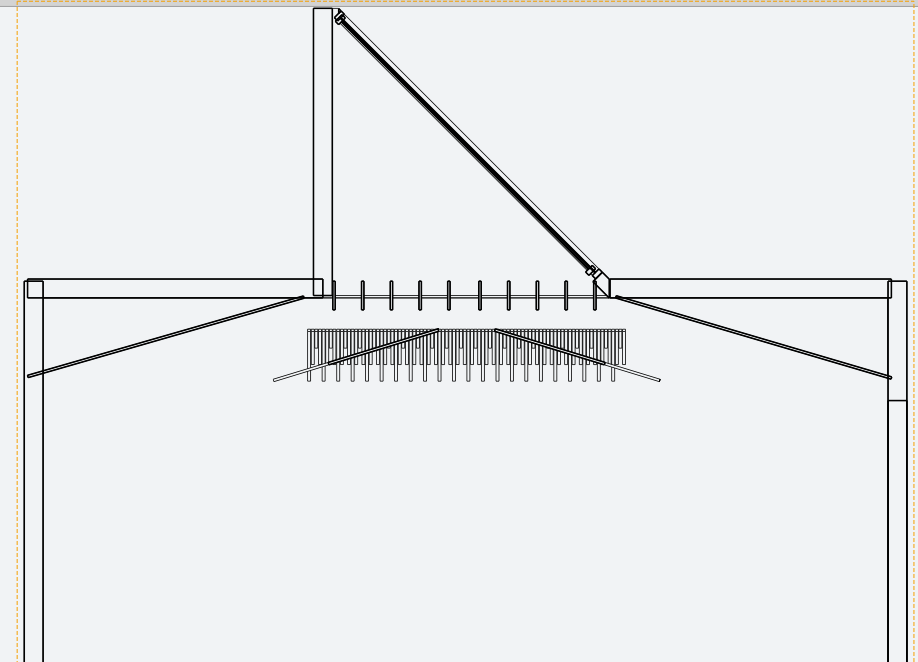
\includegraphics[width=0.45\linewidth]{archetecturesegment.png}
            \caption{After the first modification}
            \label{fig:placeholder}
        \end{figure}
      \end{itemize}
    \end{frame}


    \subsection{Second Modification}
    \begin{frame}{Second Modification}
      \framesubtitle{Cutting the light down to range}
      \begin{itemize}
        \item Even after the angle change the room still received nearly double the target illumination
        \item \textbf{Attempt 1:} increase reflector density to reflect less light -- not effective enough
        \item \textbf{Attempt 2:} decrease reflector reflectivity -- made dark spots
        \item \textbf{Final fix:} reduce the skylight's surface area
        \begin{itemize}
            \item Trial and Error
            \item             reduced by 50\% -- too much
            \item             reduced by 30\% -- too much
        \end{itemize}
      \end{itemize}

    \end{frame}

    \begin{frame}{Final Fix}
        \begin{itemize}
          \item[ ] Compared Santa Fe to Mt' Angel for the right reduction 
          \item[] Mount Angel design transmitted about 72\% of available sky light
          \item[]Santa Fe's target required about 58\% transmission
          \item[] Skylight area reduced from 100 ft$^2$ to 80 ft$^2$ (a 20\% cut)
        \end{itemize}
        \begin{figure}
            \centering
            \includegraphics[width=0.5\linewidth]{finalsectionview.png}
            \caption{Final Design}
            \label{fig:placeholder}
        \end{figure}
        \item This kept the room within range even at Santa Fe's brightest measured illumination, 12,100 fc
    \end{frame}
        

    %%%%%&%%&\end{frame}

    \section{Results}
    \begin{frame}{Results}
      \framesubtitle{Final design}
      \begin{itemize}
        \item Final design: a 70\textdegree, north-facing, 8 ft $\times$ 10 ft skylight with louvers and reflectors, transmitting 58\% of available sky light
        \item Average daylight factor: 3.8\% with louvers fully open, 0.3\% with louvers fully closed
        \item Room stays within the 20-45 fc target range across the full range of outside light -- from about 500 fc up to 12,100 fc
      \end{itemize}
      \begin{figure}
          \centering
          \includegraphics[width=0.55\linewidth]{Finallightstdy.png}
          \caption{Final light study, FC}
          \label{fig:placeholder}
      \end{figure}
    \end{frame}
    

    \begin{frame}{Results}
      \framesubtitle{Generalizing to other climates}
      \begin{itemize}
        \item Reflector set should replicate the original's properties (glass, fabric, or panel materials all viable) and span about 16\% of the room's area from the center opening
        \item Keep a 16 in gap between the reflectors/louvers and the skylight opening
        \item Tilt the skylight toward north in the northern hemisphere at an angle slightly less than the location's maximum solar altitude, to control light intensity
      \end{itemize}
    \end{frame}

    \begin{frame}[label=bibliography]{Sources}
      \begin{thebibliography}{9}
        \bibitem{dekay}
            Mark~DeKay and G.~Z.~Brown.
            \emph{Sun, Wind, and Light: Architectural Design Strategies}, 3rd ed.

        \bibitem{mazria}
            Edward~Mazria.
            \emph{The Passive Solar Energy Book}.

        \bibitem{uoregon}
            Energy Studies, University of Oregon.

        \bibitem{velux}
            Velux.
            \emph{Daylight Calculations and Measurements}.
            \url{https://www.velux.com/healthy-buildings/research-and-knowledge/deic-basic-book/daylight/daylight-calculations-and-measurements}

        \bibitem{timeanddate}
            \emph{Sun -- Santa Fe, New Mexico}.
            \url{https://www.timeanddate.com/sun/usa/santa-fe}

        \bibitem{healio}
            \emph{The Physics of Light}.
            \url{https://www.healio.com/news/ophthalmology/20120331/the-physics-of-light}
      \end{thebibliography}
    \end{frame}

\end{document}